\section{Where the rent moves: contestable execution and the economics of settlement capital}
\label{sec:rent}

The previous sections located a scarce resource, directional capital on a cut, and asked how settlement objects relocate it. This section asks the commercial version of the question for a derivatives market. If execution is decentralized, so that independent routers run private books and consume substitutable price feeds, does scarcity, and with it the revenue a protocol can defend, move into settlement capital? And can a protocol pay the suppliers of that capital without recreating the centralized bottleneck it removed? The application is SatsHedgeZero (SHZ), a design for BTC-settled derivatives in which independent routers match signed orders against locally allocated collateral, a federation of five signers certifies one price packet every 200\,ms, fills are batched into 100\,ms Lightning commitments, and contracts settle as discreet log contracts (DLCs) with an explicit zero settlement fee.

\subsection{Execution rent and why it does not survive contestability}
\label{sec:rent-exec}

A centralized venue that controls a sequencer controls access to the liquidity resting behind it, and can price that access. Lighter, an order-book exchange on a zero-knowledge rollup, does so: its standard accounts pay nothing and wait 300\,ms, its premium accounts pay up to 2.8\,bp per taker fill and wait 140\,ms. A companion study replays 1{,}920 sequence-verified hours of its public BTC, ETH and SOL books \citep{dugan2026latency}. It finds that the fee is not paying for the latency advantage: averaged over all decisions, moving a taker from 300 to 100\,ms saves 0.009--0.021\,bp, no causal policy beats free execution out of sample, and per-trade fees reconciled to the venue's published revenue are 0.75\,bp of volume, of which makers, who supply the resting liquidity, pay 37 percent. The rent is in access to a concentrated book, not in time. Whether it survives decentralization is the question of contestable markets \citep{baumol1982contestable}: a market served by firms that can enter and leave without sunk cost prices at average cost whatever the number of incumbents, and what protects a markup is a sunk cost or a switching cost \citep{klemperer1987switching}.

\begin{proposition}[contestable execution]
\label{prop:contest}
Let $n\ge 2$ routers offer the same execution service, against the same depth, latency and safety, at a constant marginal cost $c$, with no capacity limit, and let customers buy from a lowest-price router. With zero switching cost any common price $p>c$ admits a strictly profitable undercut. A customer who pays a switching cost $\sigma\ge 0$ to leave its incumbent stays only if $p\le c+\sigma$, so the sustainable execution markup is at most $\sigma$.
\end{proposition}

Both statements are proved in Lean (\texttt{undercut\_\allowbreak{}profitable}, \texttt{sustainable\_\allowbreak{}markup} in \texttt{formal-rent/\allowbreak{}SpiralRent/\allowbreak{}Contest.lean}). The proposition is conditional, and each condition is an attack surface for the rent. Distinct liquidity, exclusive order flow and a licensed feed are differentiation; a book of resting orders is not substitutable in the way a price observation is. What the proposition does say is that a router whose product is the oracle packet it republishes, or the 200\,ms by which it republishes it early, has nothing to charge for once a second router receives the same packet. In SHZ the packet is common by construction, signed by the federation and released to every subscriber under the same terms. The companion study adds that even the early packet's value is a transfer: a subscriber who sees the mark 200\,ms ahead profits only by taking stale quotes from makers, and no per-fill rebate from the same trade covers the maker's loss. The execution layer therefore earns at most the switching cost plus the value of whatever liquidity it can make exclusive, and a design that wants to avoid a bottleneck must make liquidity non-exclusive.

\subsection{The resources that remain scarce}
\label{sec:rent-scarce}

What competition among routers does not compress is anything with a capacity, a clock or a bond. Settlement on Bitcoin consumes five such resources. \emph{Directional Lightning liquidity} is the stock of Lemma~\ref{lem:cut}: a payout to a creditor needs capacity toward that creditor, forecast in advance and placed per edge. \emph{Collateral fronting} is the stock $W_S$ of Proposition~\ref{prop:relocation}: value advanced to one party before it is recovered from another. \emph{Enforceable settlement rights} are the authority field of the settlement object: a claim is worth its face value only if some path pays it without the debtor's cooperation. \emph{Multilateral netting} reduces settlement flows \citep{duffie2011ccp} but, as Section~\ref{sec:rent-netting} shows, not the collateral that backs open positions. \emph{Proof and dispute capital} is the escrow of Proposition~\ref{prop:bond}: an operator bond and a challenge period, during which whatever the statement releases stays locked.

\begin{definition}[competitive return and rent]
A supplier of a resource earns a competitive return when its revenue equals its costs including the opportunity cost $r$ of the capital it commits, $\int r K(t)\,dt$, plus a premium for the risks it bears. Economic rent is revenue in excess of that sum. Rent requires a scarce input whose supply cannot be expanded at the competitive price within the horizon: a capacity, an entry lag, a sunk setup, or a bargaining position.
\end{definition}

Settlement capital earns a competitive return wherever new capital can arrive at cost $r$; it earns a rent only while capacity binds and before new capital can be placed. The clocks of Table~\ref{tab:objects} are entry lags: a channel needs confirmations, a BitVM3 setup needs hours of garbling and a committee, a bond must be posted on chain. The question is therefore empirical: how much capital each architecture locks, for how long, who owns it, what a constraint on it is worth, and how fast a competitor could supply more.

\subsection{Settlement capital as an inventory of objects}
\label{sec:rent-inventory}

We extend the liquidity duration of Section~\ref{sec:ratio} to derivatives. Fix a horizon, a trade history and, for each trade, a contract: a fixed-maturity inverse BTC/USD position between a taker and a maker, notional $q$ in USD, entry price $P_0$, leverage $L$, so that each side posts margin $m=q/(LP_0)$ BTC. At maturity $T$ the long side's payoff $q(1/P_0-1/P_T)$ is clipped to $[-m,m]$, the most a DLC funded by $m$ per side can pay, and the debtor owes the creditor the clipped amount. Every satoshi backing an enforceable object is inventoried once at each instant as an object with an amount, an owner, a category, a lock time, a release time and a verification class: the mechanism whose observation would establish that spend authority has been restored. Peak locked capital is the maximum of the inventory, integrated locked capital $\mathcal K=\int K(t)\,dt$ is in BTC-days, and $\mathcal K/V$, with $V$ the matched notional in BTC, is the capital duration. A pending obligation already backed by counted collateral is not counted again, and fees are transfers, not resource costs.

Five architectures are compared on identical demand, contracts and price paths. \textbf{A}, independent bilateral LN-DLC settlement: each taker--maker pair holds a channel provisioned at the peak of its concurrent margins and released at maturity, or after the unilateral exit delay when a counterparty is offline. \textbf{B}, router-local netting: each trader holds one channel per router, provisioned at its peak margin there; settlement nets per router batch; the router operator provisions, per channel, the running maximum of the trader's cumulative net receipts, which is Lemma~\ref{lem:cut} on the cut around that trader. \textbf{C}, UTXORef multilateral clearing: margins sit in vault outputs, every round of length $P_s$ nets the matured obligations of all parties, and payouts leave the vaults in one clearing transaction subject to a restricted payout graph (Section~\ref{sec:rent-cut}); margin is reusable once that transaction has three confirmations. \textbf{D}, C with LP-funded advances: at maturity an LP pays every customer over Lightning, returning margins as well as winnings, and is reimbursed from the vaults once the batch's clearing statement has been proven and the BitVM3 challenge period has passed, against an operator bond of half the LP's peak advance. \textbf{E}, unrestricted frictionless clearing: release exactly at maturity with no delay, bytes or proofs, a theoretical control. Three further rows replace per-contract margin by pre-maturity portfolio margin: per trader and router (\textbf{B\_pm}), per trader across routers (\textbf{C\_pm}, \textbf{E\_pm}).

The proof work in D is transparent end to end: a Nova folding proof \citep{kothari2022nova} over the batch's obligations, attested inside an SP1 guest whose compressed proof uses a BLAKE3 final layer, and checked by a garbled-circuit verifier of 785 million gates that garbles and evaluates in 209\,s \citep{spiral2026}. The guest that verifies a Nova proof executes about $2.1\times10^{10}$ instructions; we charge three GPU-hours at \$1.50 per batch. No Groth16 circuit and no trusted setup is part of the proposed SHZ settlement path, which removes for D the third trust assumption of Section~\ref{sec:limits}; the BitVM3 committee assumption remains. The on-chain footprint we charge is a 300\,vB claim per batch and, with probability $0.01$, the published Assert and Disprove sizes.

\subsection{Netting moves flows, not margin}
\label{sec:rent-netting}

For matured obligations $g_{ij}\ge0$ write $b_i=\sum_j g_{ji}-\sum_j g_{ij}$, $G=\sum_{ij}g_{ij}$ and $N=\sum_i\max(b_i,0)$.

\begin{proposition}[netting bound]
\label{prop:netting}
$\sum_i b_i=0$, $N=\tfrac12\sum_i|b_i|$, and $N\le G$. Netting is a statement about payment at maturity: an obligation set with $G>0$ and $N=0$ exists, and nothing in it releases the collateral of unexpired contracts.
\end{proposition}

The Lean proofs are \texttt{sum\_\allowbreak{}netPos}, \texttt{netFlow\_\allowbreak{}eq\_\allowbreak{}half\_\allowbreak{}abs}, \texttt{netFlow\_\allowbreak{}le\_\allowbreak{}gross} and the counterexample \texttt{netting\_\allowbreak{}zero\_\allowbreak{}flow}. The experiment bears the distinction out. In the base cell, multilateral netting reduces settlement flow from $G=82.8$ to $N=32.4$\,BTC, by 61 percent, and router-local netting to 31.8. Neither changes the margin that backs open positions. The frictionless control E locks exactly $2mT$ per contract, $0.200$ BTC-days per BTC matched at $L=10$ and $T=24$\,h, and every per-contract-margin architecture lies above it. The correlation of traders' directional biases, swept from 0 to 1, changes net flows and leaves per-contract capital unchanged to the last digit, because a DLC's margin does not depend on which side is crowded. Capital falls below $2mT$ only when the collateral rule changes, to portfolio margin, and then a separate risk statement is needed (Section~\ref{sec:rent-pm}).

\subsection{The restricted payout graph}
\label{sec:rent-cut}

A clearing round pays creditors $j$ amounts $d_j$ from vault budgets $C_v$ along payout edges of capacity $u_{vj}$, absent where a vault cannot pay a creditor directly (different routers, scripts, or channel topology). A payout $x$ is feasible if $0\le x_{vj}\le u_{vj}$ and $\sum_j x_{vj}\le C_v$, and delivers fully if $\sum_v x_{vj}=d_j$.

\begin{proposition}[payout cut condition]
\label{prop:payoutcut}
Full delivery implies, for every creditor set $S$,
\[
\sum_{j\in S}d_j\;\le\;\sum_v\min\Big(C_v,\;\sum_{j\in S}u_{vj}\Big),
\]
so a violated inequality certifies a deficit. The condition is sufficient for a single vault, and for any number of vaults when every edge can carry its creditor's demand and total budget covers total demand.
\end{proposition}

{\sloppy Necessity, the deficit certificate and both sufficiency cases are proved in Lean (\texttt{cut\_\allowbreak{}necessary}, \texttt{deficit\_\allowbreak{}of\_\allowbreak{}cut}, \texttt{cut\_\allowbreak{}sufficient\_\allowbreak{}single\_\allowbreak{}vault}, \texttt{cut\_\allowbreak{}sufficient\_\allowbreak{}unrestricted}). General sufficiency is max-flow/min-cut \citep{fordfulkerson1956} on the three-layer network and is not formalized; the experiment's tests check on random instances that the undelivered amount equals the worst cut violation. The condition is the cut bound of Lemma~\ref{lem:cut} again, now on a bipartite graph whose left side is collateral and whose right side is claims: a clearing round can net any amount of obligation flow and still fail to pay a creditor whose vaults lack edges to it.\par}

\subsection{Release, authentication and enforceable claims}
\label{sec:rent-release}

Capital savings count only if customers' claims survive them. Let a state hold, per party $p$, locked collateral, free balance, and matured claims $c_{pq}$ that $p$ owes $q$. Admit two release transitions, each requiring an authenticated statement (in SHZ, a verified clearing statement): paying at most $c_{pq}$ from $p$'s collateral to $q$, and returning to $p$ only the excess of its collateral over its outstanding claims.

\begin{proposition}[conservation under authenticated release]
\label{prop:release}
Along any history of such transitions, total value $\sum_p(\text{locked}_p+\text{free}_p)$ is conserved, the backing invariant $\sum_q c_{pq}\le\text{locked}_p$ is preserved for every party, and every increase of a free balance is witnessed by an authenticated statement.
\end{proposition}

The Lean statements are \texttt{step\_\allowbreak{}conserves}, \texttt{step\_\allowbreak{}preserves\_\allowbreak{}backing}, \texttt{free\_\allowbreak{}increase\_\allowbreak{}authenticated} and \texttt{history\_\allowbreak{}invariants}. The proposition draws the line this section needs between simulated and verified release. Every release in the experiment is simulated. Each is tagged with the mechanism that would verify it: a channel state, a confirmed clearing transaction, an LP's Lightning payment, or an LP's reimbursement after proof and challenge. The proposition holds of a system that releases only through authenticated transitions, and says nothing about a simulator that records a release without one. The Testnet4 campaign of the companion branch measured one verified case: a payer's change became spendable again two blocks after its settlement transaction was submitted, 29 and 38 minutes on the two settlements of the pilot. The SHZ reference router, by its own documentation, keeps committed DLC margin encumbered and implements no DLC closure or withdrawal. Until one is implemented and observed, D's customer release at maturity is a scenario.

\subsection{Fee feasibility}
\label{sec:rent-fee}

Let $C_{0U}$ be customers' all-in cost under a baseline architecture, $C_{1U}$ their cost under a candidate before its service fee $F$, and $C_{1P}$ the provider's incremental cost, including its own capital carry, proofs, bytes and bonds, on the same horizon and numeraire.

\begin{proposition}[fee ceiling]
\label{prop:fee}
A fee satisfying aggregate customer participation $C_{1U}+F\le C_{0U}$ and non-negative provider economic profit $F\ge C_{1P}$ exists if and only if $C_{1P}\le C_{0U}-C_{1U}$, and the provider's profit is at most $C_{0U}-C_{1U}-C_{1P}$. Individual participation implies the aggregate condition and not conversely.
\end{proposition}

The Lean proofs are \texttt{fee\_\allowbreak{}feasible\_\allowbreak{}iff}, \texttt{profit\_\allowbreak{}le\_\allowbreak{}surplus}, \texttt{individual\_\allowbreak{}implies\_\allowbreak{}aggregate} and the counterexample \texttt{aggregate\_\allowbreak{}not\_\allowbreak{}individual}. With a common funding rate $r$, saved capital $\Delta\mathcal K$ in BTC-days and other customer savings $\Delta O$, the ceiling in basis points is $10^4(r\Delta\mathcal K/365+\Delta O)/V$, monotone in $r$ (\texttt{ceilingBps\_\allowbreak{}mono\_\allowbreak{}rate}). The ceiling bounds what a customer will pay; it is not revenue, and it is not the provider's profit.

\subsection{Experiment CBM-SHZ-01}
\label{sec:rent-exp}

Demand timing and volatility come from 67 days of public Lighter BTC trades (2026-09-16 to 11-21): an intraday intensity profile, the day's mean trade size and the one-minute return distribution, whose standard deviation runs from 1.7\,bp on the calmest day to 12.8\,bp on the most volatile. Synthetic paths draw Student-$t$ minute returns matched to a regime's volatility and kurtosis; an empirical cell replays a week of local Lighter prices instead. The base cell has 200 traders with Pareto activity and directional biases of correlation $0.3$, 8 makers quoting on every one of 4 routers, \$20\,M of daily volume for seven days (607{,}000 contracts, $V=6{,}843$ BTC), leverage 10, 24-hour maturity, one-hour clearing rounds, 5 percent of parties offline on any day, BTC funding at 5 percent a year for traders and LPs, 10\,sat/vB, a 144-block challenge period and one proof batch per hour. Participant collateral, channel topology and offline behaviour are assumptions; the L2 data constrain timing and prices, not anyone's inventory. Table~\ref{tab:rent} gives the base cell over three seeds, and Figures~\ref{fig:rentcap}--\ref{fig:rentsweep} give the sweeps.

\begin{table}[t]
\centering
\small
\setlength{\tabcolsep}{4pt}
\begin{tabular}{@{}lrrrrrrrr@{}}
\toprule
 & Peak & $\mathcal K$ & $\mathcal K/V$ & Reuse & $N/G$ & Fee & Provider & Surplus \\
 & BTC & BTC-days & days & h (mean) & & ceiling bp & cost bp & bp \\
\midrule
A bilateral LN-DLC & 442 & 4{,}166 & 0.58 & 2.3 & 1.00 & -- & -- & -- \\
B router-local & 316 & 3{,}124 & 0.42 & 2.8 & 0.38 & 0.35 & 0.02 & 0.33 \\
C multilateral & 256 & 1{,}632 & 0.23 & 3.3 & 0.39 & 0.70 & 0.29 & 0.40 \\
D C + LP advance & 643 & 4{,}633 & 0.65 & 0.0 & 0.39 & 0.74 & 0.93 & $-0.20$ \\
E frictionless & 205 & 1{,}398 & 0.20 & 0.0 & 0.39 & 0.74 & 0 & 0.74 \\
\midrule
B\_pm & 49 & 522 & 0.06 & 2.8 & 0.38 & 0.84 & 0.02 & 0.82 \\
C\_pm & 35 & 237 & 0.03 & 3.3 & 0.39 & 0.97 & 0.29 & 0.68 \\
\bottomrule
\end{tabular}
\caption{CBM-SHZ-01 base cell, mean of three seeds for $\mathcal K$ (standard deviation 29--201 BTC-days). Fee ceiling, provider cost and surplus are relative to A, in bp of matched notional. Under D the customer's capital is released at maturity, a simulated release; the LP is reimbursed after 28.0\,h (median) and 52.9\,h (99th percentile). B\_pm impairs 0.063 BTC of claims that per-contract margin would have paid.}
\label{tab:rent}
\end{table}

\begin{figure}[t]
\centering
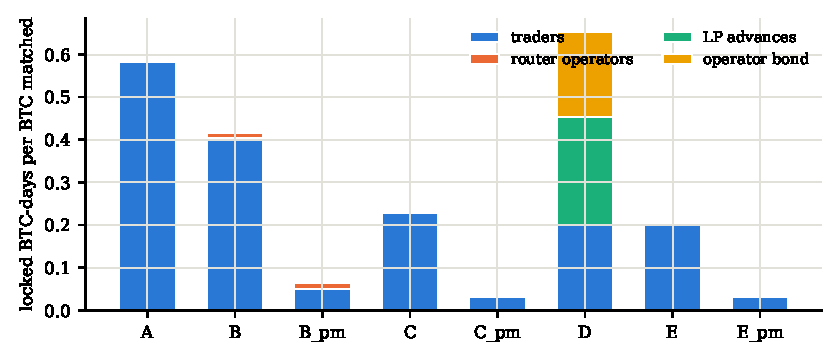
\includegraphics[width=0.85\textwidth]{figs_rent/capital_by_arch.pdf}
\caption{Locked BTC-days per BTC matched, by owner, base cell. D moves customer capital to an LP and an operator bond and locks more in total than it frees.}
\label{fig:rentcap}
\end{figure}

\paragraph{Where the capital saving comes from.} C locks 39 percent of A's BTC-time (38 percent on the empirical replay), and E 34 percent. Almost all of C's saving is the removal of idle channel provisioning, the per-edge forecast of Section~\ref{sec:lightning}: A provisions each taker--maker channel at the peak of its concurrent margin for its whole life, and C locks each margin only while its contract is open. Netting contributes the flow reduction of Proposition~\ref{prop:netting} and nothing to pre-maturity capital. C's remaining distance to E is its release clock, the round boundary plus three confirmations, and the unilateral exits of offline parties.

\paragraph{The clearing fee.} C is feasible in the base cell. Its customers save 0.70\,bp of matched notional, its provider spends 0.29\,bp (almost all of it clearing-transaction bytes), and the surplus is 0.40\,bp. Expressed per unit of capital, the ceiling is 19{,}700\,sat per BTC-day saved against a competitive rental of 13{,}700 at 5 percent. Figure~\ref{fig:rentfee} shows where feasibility ends. At a funding rate of 0.25 percent the ceiling falls to 0.24\,bp against a provider cost of 0.29, and at 1 percent the two cross. At 200\,sat/vB the clearing bytes cost 5.87\,bp against a ceiling of 4.76. The ceiling scales with the capital duration it saves: it is 2.32\,bp at 168-hour maturity, 2.64\,bp at leverage 2 and 0.46\,bp at leverage 20. Fixed costs dominate small markets. At \$1\,M a day the provider cost is 2.39\,bp against a ceiling of 3.81; at \$100\,M it is 0.06 against 0.36.

\begin{figure}[t]
\centering
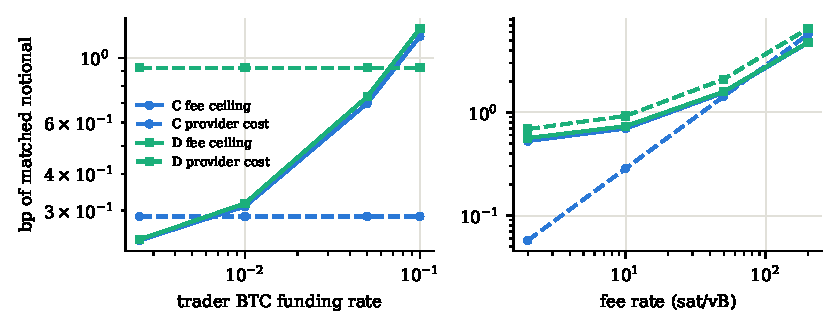
\includegraphics[width=0.85\textwidth]{figs_rent/fee_feasibility.pdf}
\caption{Fee ceiling (solid) against provider cost (dashed) for C and D across the trader funding rate (left; the LP rate is held at 5 percent) and the Bitcoin fee rate (right). The clearing service is feasible where the solid line lies above the dashed one.}
\label{fig:rentfee}
\end{figure}

\paragraph{The settlement-credit counterexample.} D releases customer capital at maturity and pays for it with LP capital locked over the proof latency and the challenge period. In the base cell it frees 188 customer BTC-days relative to C and locks 1{,}729 LP BTC-days and 1{,}371 bond BTC-days: total capital rises 11 percent above A, and the provider's cost (0.93\,bp) exceeds the customers' ceiling (0.74\,bp). The same holds on the empirical replay (surplus $-0.14$\,bp). Valued at the customers' own funding rate, the freed capital would pay the LP 0.3 percent a year on what it commits. Figure~\ref{fig:rentsweep} (left) shows the dependence on the challenge period: D locks 0.58 of A's BTC-time at 6 blocks, 0.69 at 36, 1.12 at 144 and 5.30 at 1{,}008. An advance funded across a dispute window longer than the clearing delay it removes relocates capital and adds to it. D becomes feasible where the window is short (surplus 0.28\,bp at 6 blocks and 0.11\,bp at 36), where the capital it frees is long-lived (1.45\,bp at 168-hour maturity), or where it advances payouts but not margin returns (0.37\,bp, with capital close to C's).

\begin{figure}[t]
\centering
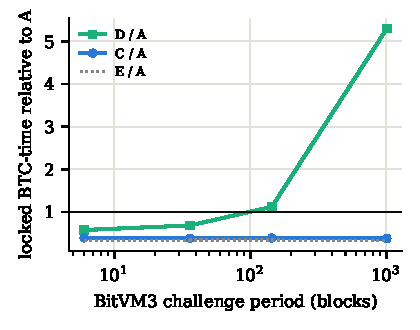
\includegraphics[width=0.42\textwidth]{figs_rent/challenge_period.pdf}\hfill
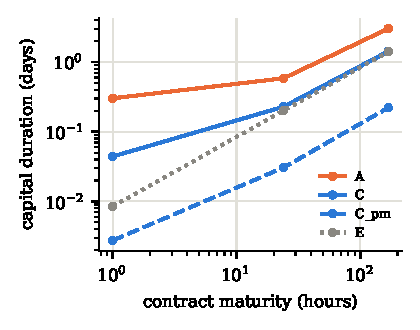
\includegraphics[width=0.42\textwidth]{figs_rent/maturity.pdf}
\caption{Left: locked BTC-time relative to A against the BitVM3 challenge period. Right: capital duration against contract maturity for A, C, C under portfolio margin, and E.}
\label{fig:rentsweep}
\end{figure}

\paragraph{Portfolio margin and impaired claims.}\label{sec:rent-pm} Portfolio margin, charging net exposure plus mark-to-market losses with variation margin every five minutes, cuts capital by a further 85 percent (C\_pm against C). It is not maturity netting. It changes the collateral rule, and the experiment shows the price. With 2 percent of traders failing to meet margin calls, per-router portfolio margin leaves 0.063\,BTC of claims unbacked in the base cell and 0.169\,BTC in the volatile regime, claims that per-contract margin would have paid in full. Pooling across routers (C\_pm) removes the base-cell impairment and leaves 0.024\,BTC in the volatile regime. A portfolio-margin saving is therefore claimable only with a risk statement covering the re-margining interval and gap moves, which Proposition~\ref{prop:release} does not provide, since it assumes claims are backed when they become due.

\subsection{An endogenous price for directional liquidity}
\label{sec:rent-dual}

Write the clearing round as a min-cost flow: payouts along vault-to-creditor edges at zero cost, and a deficit edge to each creditor whose cost per BTC is that of the cheapest substitute. The dual variable on a vault's budget constraint is the marginal value of one more unit of directional capacity there. It is zero wherever the constraint is slack, and when it binds it equals the substitute's cost, because the substitute is what the marginal unit displaces (complementary slackness; checked numerically in the experiment's tests, not formalized). With every payout edge present and full vault budgets, no round binds. With half the edges present, 42 of 48 rounds bind, and the shadow price is 13{,}700\,sat per BTC-day when an LP can advance the deficit at 5 percent, exactly the competitive rental. When no LP can enter and the creditor must wait for the unilateral fallback path, the price rises to 349{,}000\,sat per BTC-day, 25 times the rental.

The duals therefore are a useful endogenous price, and they answer the section's central question in one line. Directional settlement capital earns a scarcity rent only where it binds and only up to the cost of the next-best way to deliver. Free entry of LP capital caps that cost at the competitive rental, and the rent becomes a return on capital. The rents that survive are those protected by an entry lag (confirmation clocks, setup, bond posting) and they last as long as the lag.

\subsection{What the services can earn}
\label{sec:rent-services}

Priced at break-even under competitive entry, with costs including the competitive return on committed capital, the services rank as follows in the base cell.

\begin{itemize}[leftmargin=*,itemsep=1pt]
\item \emph{Directional liquidity leasing} is a rental. Router operators in B provision 93 BTC-days of directional stock. At the competitive 13{,}700\,sat per BTC-day that is 0.019\,bp per trade, earned as a return on capital and not as rent.
\item \emph{Short-duration settlement credit}, the LP advance of D, costs 0.62\,bp to supply against 0.04\,bp of customer value at a one-day challenge period, and does not pay there. It pays at 36 blocks (surplus 0.11\,bp) and at 6 (0.28\,bp), where the window is shorter than the clearing delay it removes.
\item \emph{Capital-efficient multilateral clearing} has a surplus of 0.40\,bp. Under competition the clearing fee is driven to the provider's 0.29\,bp, and the surplus goes to customers.
\item \emph{Proof generation} costs 0.011\,bp at hourly batches (168 batches at \$4.50): the verification layer is cheap per trade and is paid per batch.
\item \emph{Settlement oracle attestation}: a federation costing \$850 a day breaks even at \$8.5\,M of daily volume at 1\,bp, \$21\,M at the clearing surplus, and \$85\,M at 0.1\,bp.
\item \emph{Cross-router execution and aggregation} is contestable (Proposition~\ref{prop:contest}). Its markup is the switching cost.
\end{itemize}

Quoting in basis points per trade and in satoshis per BTC-day are not interchangeable. A bp fee scales with notional, a BTC-day price with capital-time, and the conversion factor is the capital duration $\mathcal K/V$ saved, which varies tenfold across the sweeps, from 0.18 days at leverage 20 to 1.77 at leverage 2. A clearing service that charges per trade and saves capital per day overcharges short-dated, highly levered flow and undercharges long-dated flow. At a fixed funding rate, fee rate and volume, C's ceiling across the other 31 cells varies by a factor of 6.8 in basis points (0.39 to 2.64\,bp) and by a factor of 1.8 per unit of capital (14{,}600 to 26{,}000\,sat per BTC-day saved), close to the 13{,}700 competitive rental.

\subsection{Is the clearing network a natural monopoly?}
\label{sec:rent-monopoly}

Pooling economies would make a single clearing network cheaper than several, and a natural monopolist could then charge up to the cost of its fragmented alternative. The experiment measures three sources of such economies. Settlement flows: netting all parties across 8 routers in one pool rather than 8 independent pools reduces net flow from 3.67 to 2.84\,BTC. Fixed proof costs: one proof per batch instead of one per pool. Portfolio margin: one portfolio per trader instead of one per router, 57 rather than 69 BTC-days at 4 routers and 86 at 16. Bonds show none: the sum of the pools' peak LP advances equals the pooled peak, because maturities share one intraday profile and every pool peaks at the same minute.

The rent a single network could extract before fragmented competitors undercut it is small. Its costs rise by 0.02, 0.06 and 0.14\,bp at 2, 4 and 8 independent pools. If pools interoperate, netting parties across pools and settling pool balances with one transfer per pool per round, the rise is 0.015, 0.045 and 0.10\,bp. The rent cap is a fraction of a tenth of a basis point except where portfolio margin is pooled, and there the economy belongs to the risk model, not the network. Permissionless access to the vault format and interoperable netting bound the clearing network's rent by the interoperation cost. The rent a single network can defend is the cost of the inter-pool transfers, not the cost of the pool itself.

\subsection{What follows for decentralized market structure}
\label{sec:rent-implications}

The answer to the section's question is that decentralizing execution does move scarcity into settlement capital, and that most of what moves is a return on capital, not a rent. The cut bound of Section~\ref{sec:lightning} reappears twice: as the per-edge forecast that makes bilateral LN-DLC settlement lock 2.5 times the capital of multilateral clearing, and as the payout cut condition that limits a clearing round. The pooling of Section~\ref{sec:ark} reappears as the gap between provisioned channel stock and exact margin, and the hyperedge of Section~\ref{sec:bip448} would capture part of the same gap without a clearing provider. The proof economics of Section~\ref{sec:proofs} reappear as a cost paid per batch, cheap per trade. Their binding effect is the challenge period, which sets how long an advanced unit stays locked. The agent populations of Section~\ref{sec:agents} meet a market in which coordination among routers buys little, because execution is contestable. What a coalition could still capture is directional capacity in a market without LP entry, the 25-fold dual of Section~\ref{sec:rent-dual}, which is the stationary-placement effect of Proposition~\ref{prop:coalition} in a new setting.

A protocol can compensate its suppliers without recreating a bottleneck if it pays them as capital: per BTC-day committed, at a price that competing LPs can undercut, for capital whose release is authenticated, with permissionless vault formats and interoperable netting. It recreates the bottleneck if it pays a per-trade fee on an exclusive resource: a privileged queue, a feed whose terms differ by subscriber, or a clearing pool that will not net with others.

Four negative findings bound these conclusions. Settlement credit across a dispute window longer than the clearing delay it removes adds capital, so it should not be offered at the one-day window. Portfolio margin saves capital only with a risk statement that per-contract DLCs do not need. Clearing is infeasible below a 1 percent cost of capital or above about 50\,sat/vB. And no release in this experiment is a verified recovery of spend authority.
